\section{Literature Review}

\gls{gps} has been successful in outdoor-locating solutions, however, it cannot quite repeat this success indoors. Since \gls{gps} signal is unable to pass through solid structures, it is impossible to be used indoors, underground and under the water. Enter the \gls{lps}, a technology that provides location information within a small coverage region. \gls{rtls} is a special type of \gls{lps} which is used to track and identify the location of an object in real time, usually within a building or other contained area.

\gls{rtls} consists of specialized receivers or readers kept at a known position which receive wireless signals from small \gls{id} batch or tag or node, attached to, or embedded in the object to be tracked. Wireless technologies include Wifi, \gls{rfid}, Infrared, Bluetooth, ultrasonic systems. These different technologies possess their own feature and are suitable for different applications. There is no all-purpose solution when it comes out to the selection of wireless technology. Tags and the fixed reference points can be transmitters, receivers or both. 

By positioning the readers or receivers at fixed know location in a given environment, the real-time location of the tags or object-to-be-tracked is determined by analyzing the different aspects of the communication between tags and readers. Most widely used techniques for these calculations are, Distance/Angle calculation, Position computation and localization. Again, the choice of method depends on the need of application. Wireless signals from a tag is received by multiple readers. Different aspect of this communication can be used to calculate the distance of the tag from different readers. Now the position of the tag is estimated using one or more locating algorithms like trilateration, multilateration, or triangulation. Finally the calculated position of the tag is displayed on a map (2D or 3D).

\gls{rtls} has been used to effectively track assets, equipment, people and animal within a predefined area. Wireless tags can be attached to the object and their location can be viewed in a map. This information is used in many applications in different fields like in inventory and asset tracking,health care, security, animal tracking, vehicle tracking.


\subsection{Wireless Technologies}

\subsubsection{\gls{ir} Based Systems}
The most prominent advantage of \gls{ir} is its wide availability since many devices are equipped with \gls{ir} sources, such as mobile phones, \gls{tv}, printer, and so forth. In addition, since the whole infrastructure is very simple, it does not need costly installation and maintenance. However, due to its requirement of line-of-sight and its inability to penetrate
opaque obstacles, it can not be applied to some kinds of indoor scenarios in which the environment is pretty complex. Besides, it is also subject to interference of other sources of \gls{ir} devices.

\subsubsection{\gls{rf} Based Systems}
\gls{rf} Based Systems Systems designed based on RF can cover larger distance since it uses electromagnetic transmission, which is able to penetrate opaque objects such as people and walls. Besides, a RF system can uniquely identify people or objects tracked in the system. Based on this technology, \gls{rtls}, \gls{wlan}, Bluetooth, wireless sensor networks, \gls{uwb} are created. In addition, RF based technologies are further divided into narrow band based technologies (\gls{rfid}, Bluetooth and \gls{wlan}) and wide band based technologies \gls{uwb}.

\gls{rfid} is technology used for identifying an object using radio waves and tags. \gls{rfid} is normally used indoors. \gls{rfid} usually uses Low Frequency, High Frequency and Ultra High Frequency. \gls{rfid} tags can be placed at the object whose position is to be located and then by using low, high or ultra high frequency signals, a communication between the receivers and the tag is established.



\subsubsection{Ultrasound Based Systems}
Ultrasonic systems can also be used in \gls{rtls} with a small coverage region. The systems based on ultrasound technology is relatively cheap and the precision is lower in comparison with \gls{ir} based systems due to the reflect influence. Additionally, this kind of systems is always associated with \gls{rf} or \gls{ir} technology to fulfill the synchronization requirement. Ultrasonic systems use ultrasonic transmitter and receivers to triangulate the position of objects. This project also uses ultrasonic system. We have made use of ultrasonic transmitters and receivers which operate at 40kHz frequency to locate the path followed by the vehicle during the trial.


\subsection{Existing Trial system}
		\gls{rtls} has been a growing field in the past few years. Extensive use of \gls{rtls} based system have shown improvement in respective area of use. As described earlier, \gls{rtls} has been in use from animal tracking to health care services. However, the complexity and cost of this system has to be taken into account before implementing this system.

		\gls{rtls} systems have been build through different techniques. But, no such system is prevalent in Nepal regarding the license trial automation system. We expect this kind of license trial system to be the first of its kind in the country.

	\subsubsection{License Trial Track}
		Recently the government of Nepal has changed the license trial system changing the track of the trial. The new trial track looks the following.
			\begin{figure}[htpb]
				\centering
				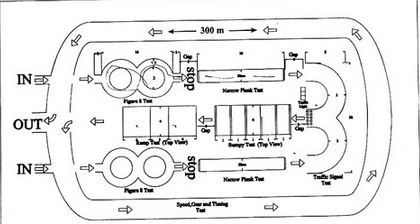
\includegraphics[scale=.75]{Images/TrialTrack.png}
				\caption{License Trial Track}
				\label{fig:LicenceTrialTrack}
			\end{figure}
		The drivers have to drive their vehicle within the permitted track following all the traffic rules and do as specified. For example they have to stop in the places written 'STOP' and do as instructed.
		
